%!xelatex = 'xelatex --halt-on-error %O %S'

\documentclass{buaaemp}
\begin{document}

% 标题,作者
\emptitle{光学运算}
\empauthor{智朝晖}{王玫}

% 奇数页页眉 % 请在这里写出第一作者以及论文题目
\fancyhead[CO]{{\footnotesize 智朝晖: 光学运算}}


%%%%%%%%%%%%%%%%%%%%%%%%%%%%%%%%%%%%%%%%%%%%%%%%%%%%%%%%%%%%%%%%
% 关键词 摘要 首页脚注
%%%%%%%%关键词
\Keyword{光学信息处理, 4f系统, 图像加减和微分, 傅里叶变换}
\twocolumn[
\begin{@twocolumnfalse}
\maketitle

%%%%%%%%摘要
\begin{empAbstract}
光学信息处理技术是指用光学方法实现对输入信息试试某种运算或变换,以达到对信息进行提取、编码、存储、增强、识别和恢复等目睹。最基本的操作是用光学方法对图像信息进行处理,并用频谱的语言来描述信息。本文利用4f系统来进行光学图像加减和图像微分处理实验,得到了图像的加减和微分图像。
\end{empAbstract}

%%%%%%%%首页角注,依次为实验时间、报告时间、学号、email
\empfirstfoot{2022-11-03}{2022-11-03}{20377365}{20377365@buaa.edu.cn}
\end{@twocolumnfalse}
]
%%%%%%%%!首页角注可能与正文重叠,请通过调整正文中第一页的\enlargethispage{-3.3cm}位置手动校准正文底部位置:
%%%%%%%%%%%%%%%%%%%%%%%%%%%%%%%%%%%%%%%%%%%%%%%%%%%%%%%%%%%%%%%%
%  正文由此开始
\wuhao 
%  分栏开始

\section{引~~言}
图像加减和微分是相干光学处理中的一种基本的光学-数学运算, 是图像识别的一种主要手段。通过相减可以求出两张相近照片的差异, 从中提取差异信息。例如:通过在不同时期拍摄的两张照片相减, 在医学上可用来发现病灶的变化; 在军事上可以发现地面军事设施的增减; 在农业上可以预测农作物的长势; 在工业上可以检查集成电路掩膜的疵病, 等等。还可用于地球资源探测、气象变化以及城市发展研究等各个领域。图像微分可以增强图像边缘较中间明亮,可以实现边缘增强,勾画轮廓识别模糊图片,(例如透过云层的卫星图片或雾中摄影图片),实现图像相减和图像微分的方法很多, 本实验利用4f系统的正弦光栅作为空间滤波器实现图像相减和微分。\cite{钱建强2016近代物理实验}

\section{原~~理}
本实验的光路系统是一个典型的相干光学处理系统(4f系统),将待处理的图像置于输入面 $P_1$的原点位置,正弦光栅的空间频率为  $f_{0}$ , 将其置于$  4 f $ 系统的滤波平面  $P_{2}$  上, 如图\ref{fig:my_label4}所示, 

\begin{figure}
    \centering
    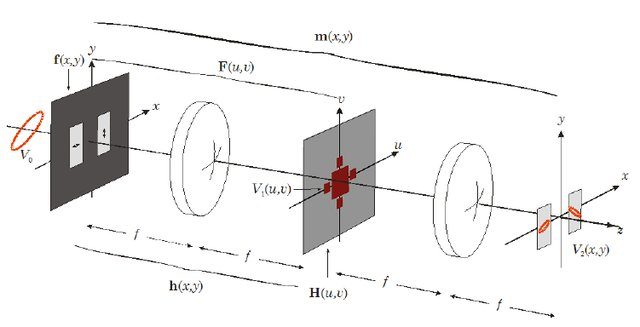
\includegraphics[width=\linewidth]{image/fourier.jpg}
    \caption{傅里叶光学4f系统}
    \label{fig:my_label4}
\end{figure}
光栅的复振幅透过率为:
\begin{align*}
    H (f_{\mathrm{x}}, \mathrm{f_y})&=\frac{1}{2}[1+\cos (2 \pi \mathrm{f}_0 \mathrm{x}_2+\phi_0)] \\
    & =\frac{1}{2}+\frac{1}{4} \mathrm{e}^{i 2 \pi \mathrm{f}_0 x_2+\phi_0}+\frac{1}{4}\mathrm{e}^{-\mathrm{i} 2 \pi \mathrm{f}_0 x_2+\phi_0} 
\end{align*}
    
\newpage

式中 $ f_{x}=x_{2} / \lambda f, f_{y}=y_{2} / \lambda f $, $ f$  为傅里叶变换透镜的焦距;  $\phi 0 $ 表示
光栅条纹的初位相, 它决定了光栅相对于坐标原点的位置。
将图像  $\mathrm{A}$  和图像 $ \mathrm{B} $ 置于输入平面 $ P_1  $上, 且沿  $x_1 $ 方向相对于坐标原点对称放置, 图像
中心与光轴的距离均为  $b $ 。选择光栅的频率为 $ f_0$ , 使得 $ b=\lambda f f_{0} $, 以保证在滤波后两图
像中A 的 $ +1$  级像和 $ \mathrm{B}$  的- 1 级像能恰好在光轴处重合。于是, 输入场分布可写成:

\begin{equation}
    f\left(x_{1}, y_{1}\right)=f_{A}\left(x_{1}-b, y_{1}\right)+f_{B}\left(x_{1}+b, y_{1}\right)
\end{equation}

在其频谱面$  P 2$  上的频谱为:
\begin{equation}
    F\left(f_{x}, f_{y}\right)=F_{A}\left(f_{x}, f_{y}\right) e^{-i 2 \pi f_{x} b}+F_{B}\left(f_{x}, f_{y}\right) e^{i 2 \pi f_{x} b}
\end{equation}

其中 $b=\lambda f f_{0} x_{2}=\lambda f f_x $,因此 $f_{x} b=f_{0} x_{2}$。上式可以写成:
\begin{equation}
    F\left(f_{x}, f_{y}\right)=F_{A}\left(f_{x}, f_{y}\right) e^{-i 2 \pi f_{0} x_{2}}+F_{B}\left(f_{x}, f_{y}\right) e^{i 2 \pi f_{0} x_{2}}
\end{equation}

经过光栅滤波后的频谱为: 

\begin{align*}
 F & \left(f_{x},   f_{y}\right) H\left(f_{x}, f_{y}\right)=  \\
& \frac{1}{4}\left[F_{A}\left(f_{x}, f_{y}\right) e^{i \phi \phi}+F_{B}\left(f_{x}, f_{y}\right) e^{-i \phi \phi}\right] + \\
& \frac{1}{2}\left[F_{A}\left(f_{x}, f_{y}\right) e^{-i 2 \pi f_{0} x_{2}}+F_{B}\left(f_{x}, f_{y}\right) e^{i 2 \pi f_{0 x_{2}}}\right]+\\
&  \frac{1}{4}\left[F_{A}\left(f_{x}, f_{y}\right) e^{-i\left(4 \pi f_{0} x_{2}+\phi\right)}+F_{B}\left(f_{x}, f_{y}\right) e^{i\left(4 \pi f_{0} x_{2}+\phi \phi_{b}\right)}\right]
\end{align*}


通过透镜$L_{2}$进行傅立叶逆变换, 在输出平面 $\mathrm{P}_{3}$上的光场为:
\begin{align*}
    g\left(x_{3}, y_{3}\right)=& \frac{1}{4} e^{t_{0}}\left[f_{A}\left(x_{3}, y_{3}\right)+f_{B}\left(x_{3}, y_{3}\right) e^{-+2 \phi}\right]+ \\ &\frac{1}{2}\left[f_{A}\left(x_{3}-b, y_{3}\right)+f_{A}\left(x_{3}+b, y_{3}\right)\right]+\\
&\frac{1}{4}\left[f_{B}\left(x_{3}-2 b, y_{3}\right) e^{-i \hbar t}+f_{B}\left(x_{3}-2 b, y_{3}\right) e^{4 \hbar}\right]
\end{align*}
即可实现加减。

经适当调整位置即可在输出面 $ \mathrm{P}_{3}$  上得到微分图形。设输入图像为 $ t(x, y)$ , 其傅里叶变换频 谱为  $T(f_x, fy)$ , 则由傅里叶变换定理有:


\begin{equation}
    F\left[\frac{\partial t(x, y)}{\partial x}\right]=i 2 \pi f_{x} T\left(f_{x}, f_{y}\right)
\end{equation}
式中$ f_{x}=x_{2} / \lambda f$, $f_{y}=y_{2} / \lambda f$ 
如果频谱面上的滤波函数为: 
\begin{equation}
    H\left(f_{x}, f_{y}\right)=i 2 \pi f_{x}=i 2 \pi\left(x_{2} / \lambda f\right)
\end{equation}

复合光栅采用全息的方法来制作。复合光棚包含了两种空间频率, 令其初始位置时的透过率函数为:

\begin{align*}
    H\left(\frac{x_{2}}{\lambda f}, \frac{y_{2}}{\lambda f}\right) = t_{0}+t_{1} \cos \left(2 \pi f_{0} x_{2}\right)+t_{2} \cos \left(2 \pi f_{0}^{\prime} x_{2}\right)
\end{align*}


\begin{align*}    
&T\left(f_{x}, f_{y}\right) H\left(f_{x}, f_{y}\right)  = \\
&T\left(\frac{x_{2}}{\lambda f}, \frac{y_{2}}{\lambda f}\right) t_{0}+\frac{t_{1}}{2} T\left(\frac{x_{2}}{\lambda f}, \frac{y_{2}}{\lambda f}\right)\left(e^{i 2 \pi f_{0} x_{2}}+e^{-i 2 \pi f_{0} x_{2}}\right) \\
&+\frac{t_{2}}{2} T\left(\frac{x_{2}}{\lambda f}, \frac{y_{2}}{\lambda f}\right)\left(e^{i 2 \pi f_{0} x_{2}}+e^{-i 2 \pi f_{0} x_{2}}\right)
\end{align*}

显然物频谱会受到两个一维余弦光栅的调制。当其受第一次记录的光栅调制后, 在输出 面  $\mathrm{P}_{3}$  上可得到 3 个衍射像, 其中零级衍射像位于 $ x_{3} \mathrm{Oy} y_{3}$  平面的原点, 正、负一级衍射像则 沿  $x_{3}$  轴对称分布于  $y_{3}$  轴两侧, 距原点的距离为  $\boldsymbol{x}_{3}=\pm \lambda \mathrm{ff}_{0}$  (  f  为透镜焦距)。同样, 受第二次记录的光栅调制后, 在输出面上将得到另一组衍射像, 其中零级衍射像仍位于坐标 原点与前一个零级像重合, 正、负一级衍射像也沿  $y_{3} $ 轴对称分布于原点两侧, 但与原点的 距离为  $x_{3}^{\prime}=\pm \lambda f f_{0}^{\prime} $ 。由于 $\Delta f_{0}=f_{0}^{\prime}-f_{0}$  很小, 故  $x 3$  与$x_{3}^{\prime}$ 的差  $\Delta x_{3}=\pm \lambda f \Delta f_{0} $ 也很小, 从而使两个对应的  $\pm 1$  级衍射像几乎重叠, 沿 $ x_{3}$  方向只 错开很小的距离  $\Delta x_{3}$  。由于  $\Delta x_{3}$  比起图形本身的尺寸要小很多,当复合光棚平林一迻 适 当的距离  $\Delta l$时, 由此引起两个同级衍射像的相移量为:

\begin{equation}
    \Delta \phi_{1}=2 \pi f_{0} \Delta l, \Delta \phi_{2}=2 \pi f_{0}^{\prime} \Delta l
\end{equation}

从而导致两个同级衍射像有一个附加的相位差
\begin{equation}
    \Delta \phi=\Delta \phi_{2}-\Delta \phi_{1}=2 \pi \Delta f_{0} \Delta l
\end{equation}
当这时两个同级衍射像正好相差π相位, 相干叠加时两者重叠部分相消, 只剩下错开的 图像边缘部分, 从而实现了边缘增强。

\section{实~~验}
本实验实验步骤如下:
\begin{enumerate}
    \item 布置好半导体激光器、扩束镜、准直镜以及4f系统,同时测量f数值,将透镜放置在焦距位置。
    \item 先进行微分处理实验,不断细调透镜以及准直镜位置,获得质量较好的微分图像。方便后续进行加减图像的实验。
    \item 将复合光栅拆卸掉换上一维光栅进行图像加减实验。
\end{enumerate}
\section{实验结果与分析}
实验结果如下,下图分别是相加后的图像,\ref{fig:my_label1},微分后的边缘增强的图像\ref{fig:my_label2},相减后的图像\ref{fig:my_label3}.
\begin{figure}
    \centering
    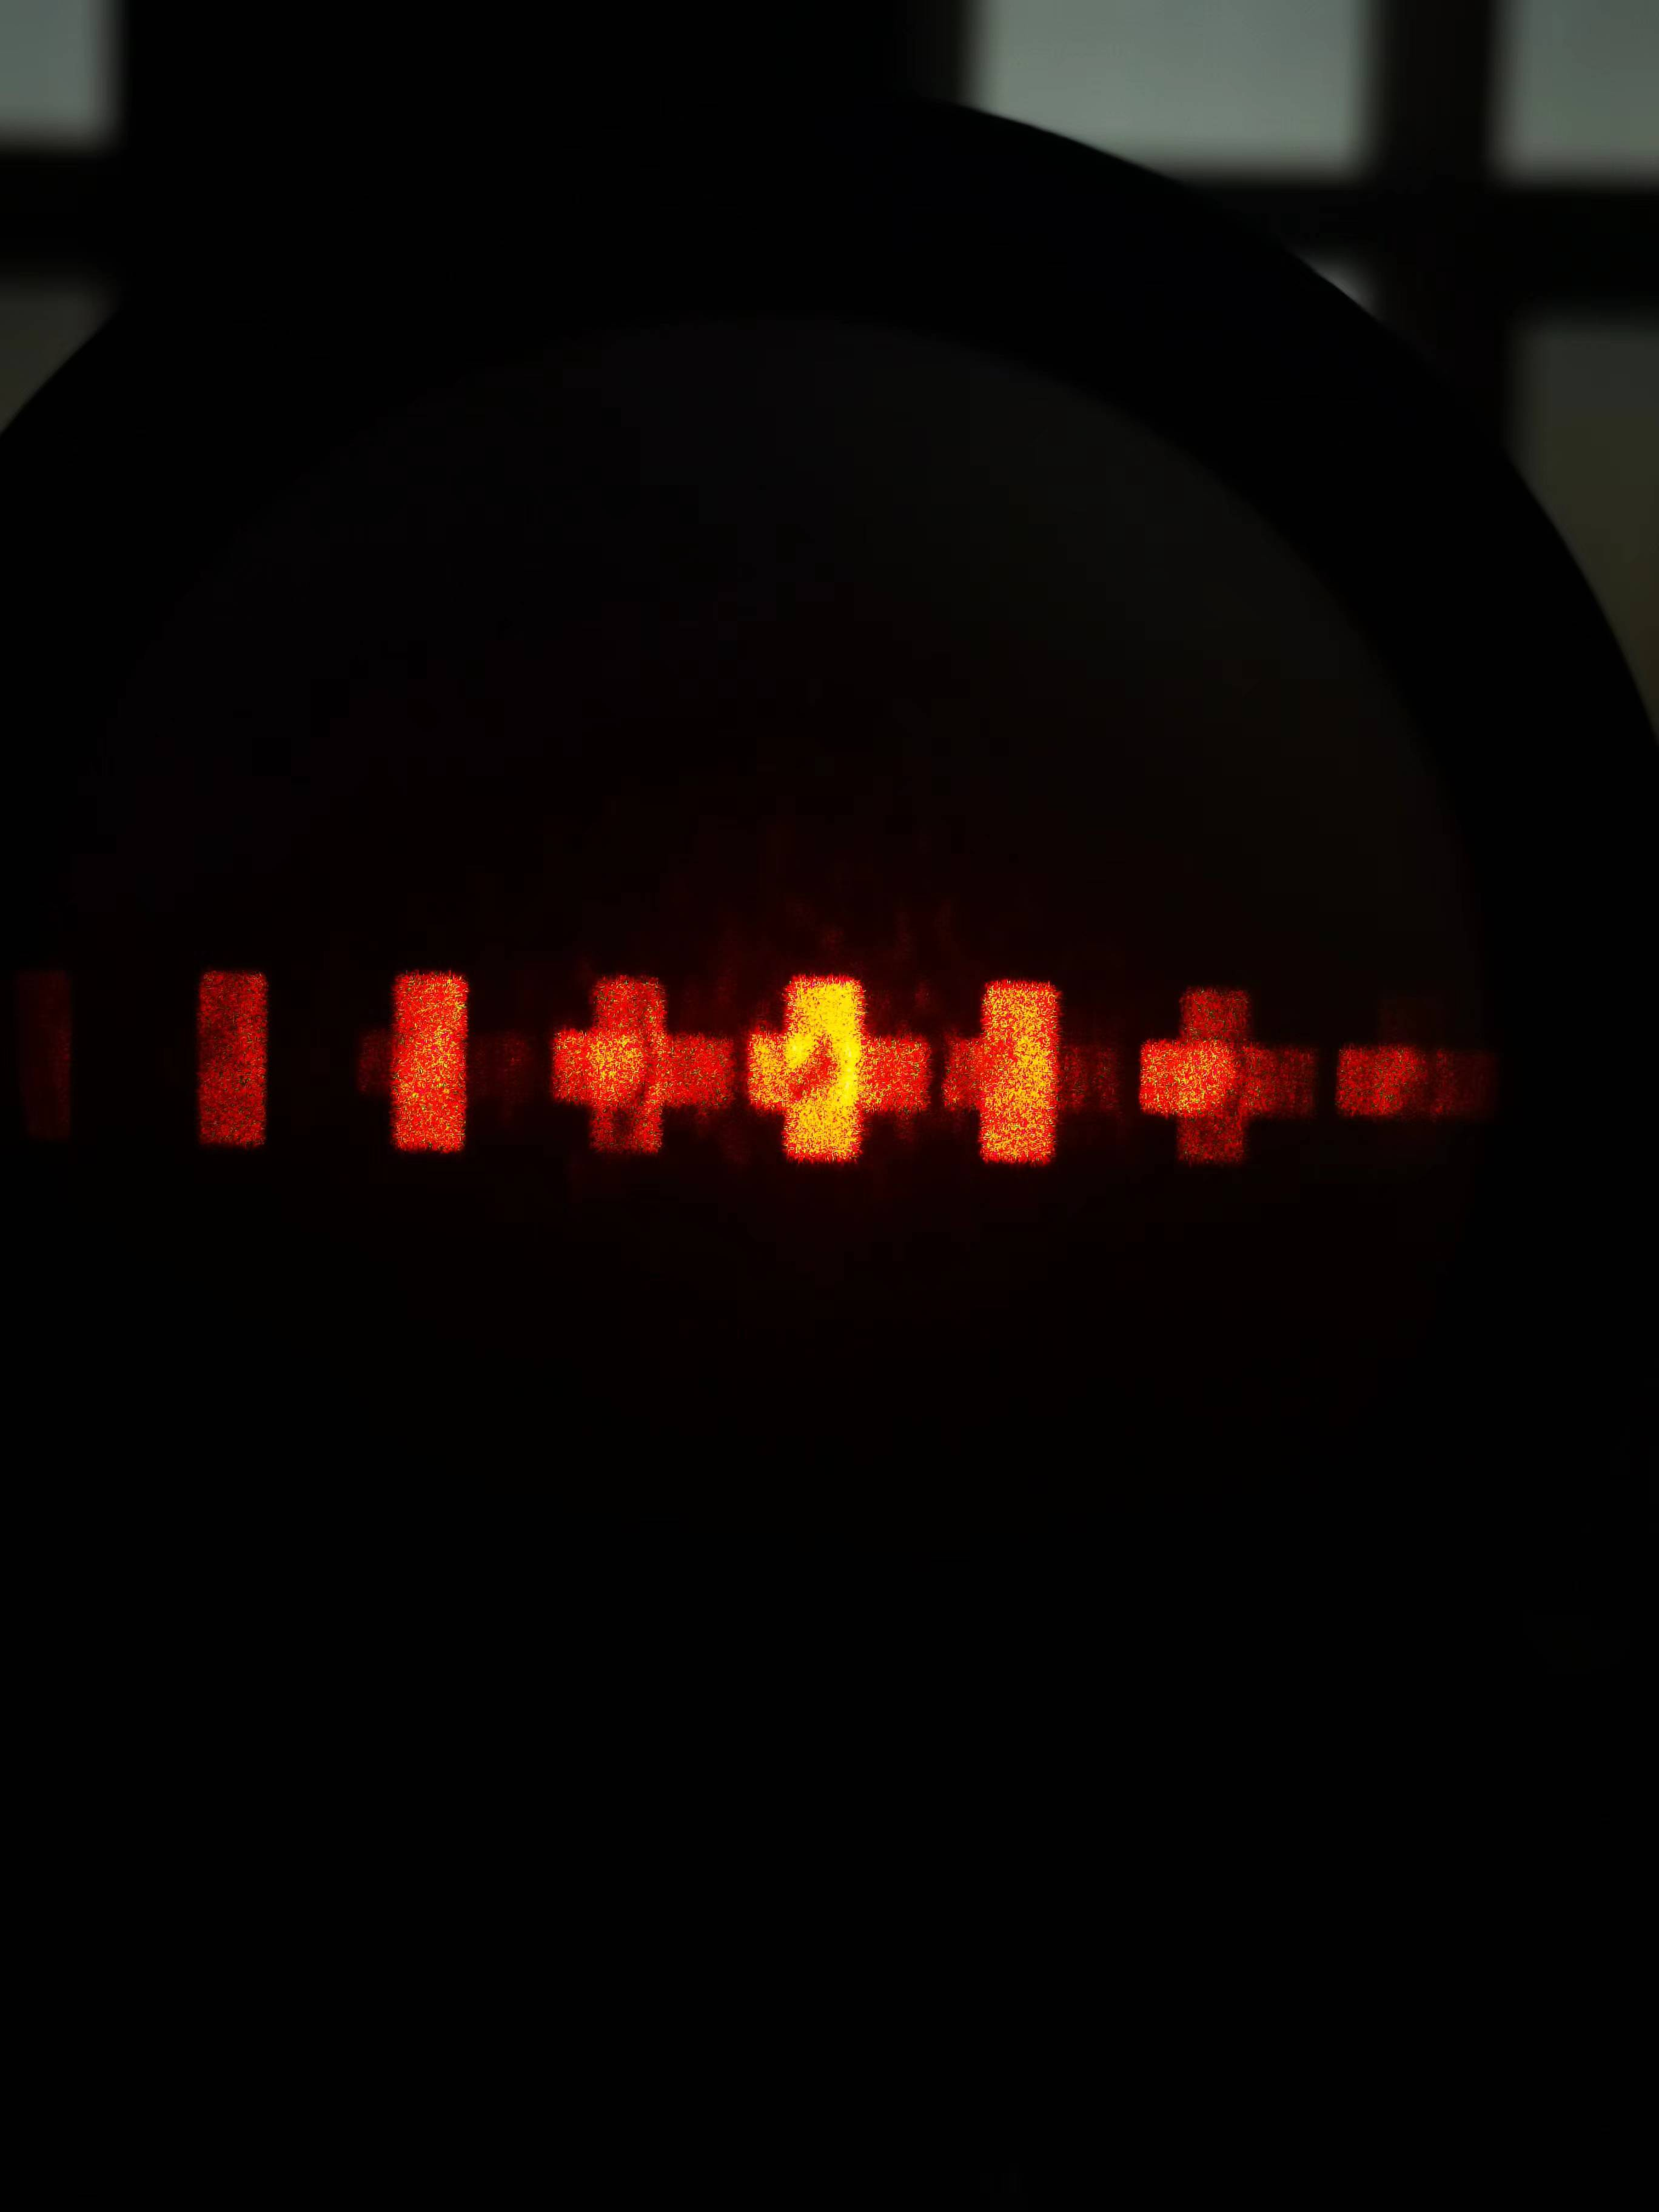
\includegraphics[width=\linewidth]{image/微信图片_20221109232920.jpg}
    \caption{相加后的图像}
    \label{fig:my_label1}
\end{figure}

\begin{figure}
    \centering
    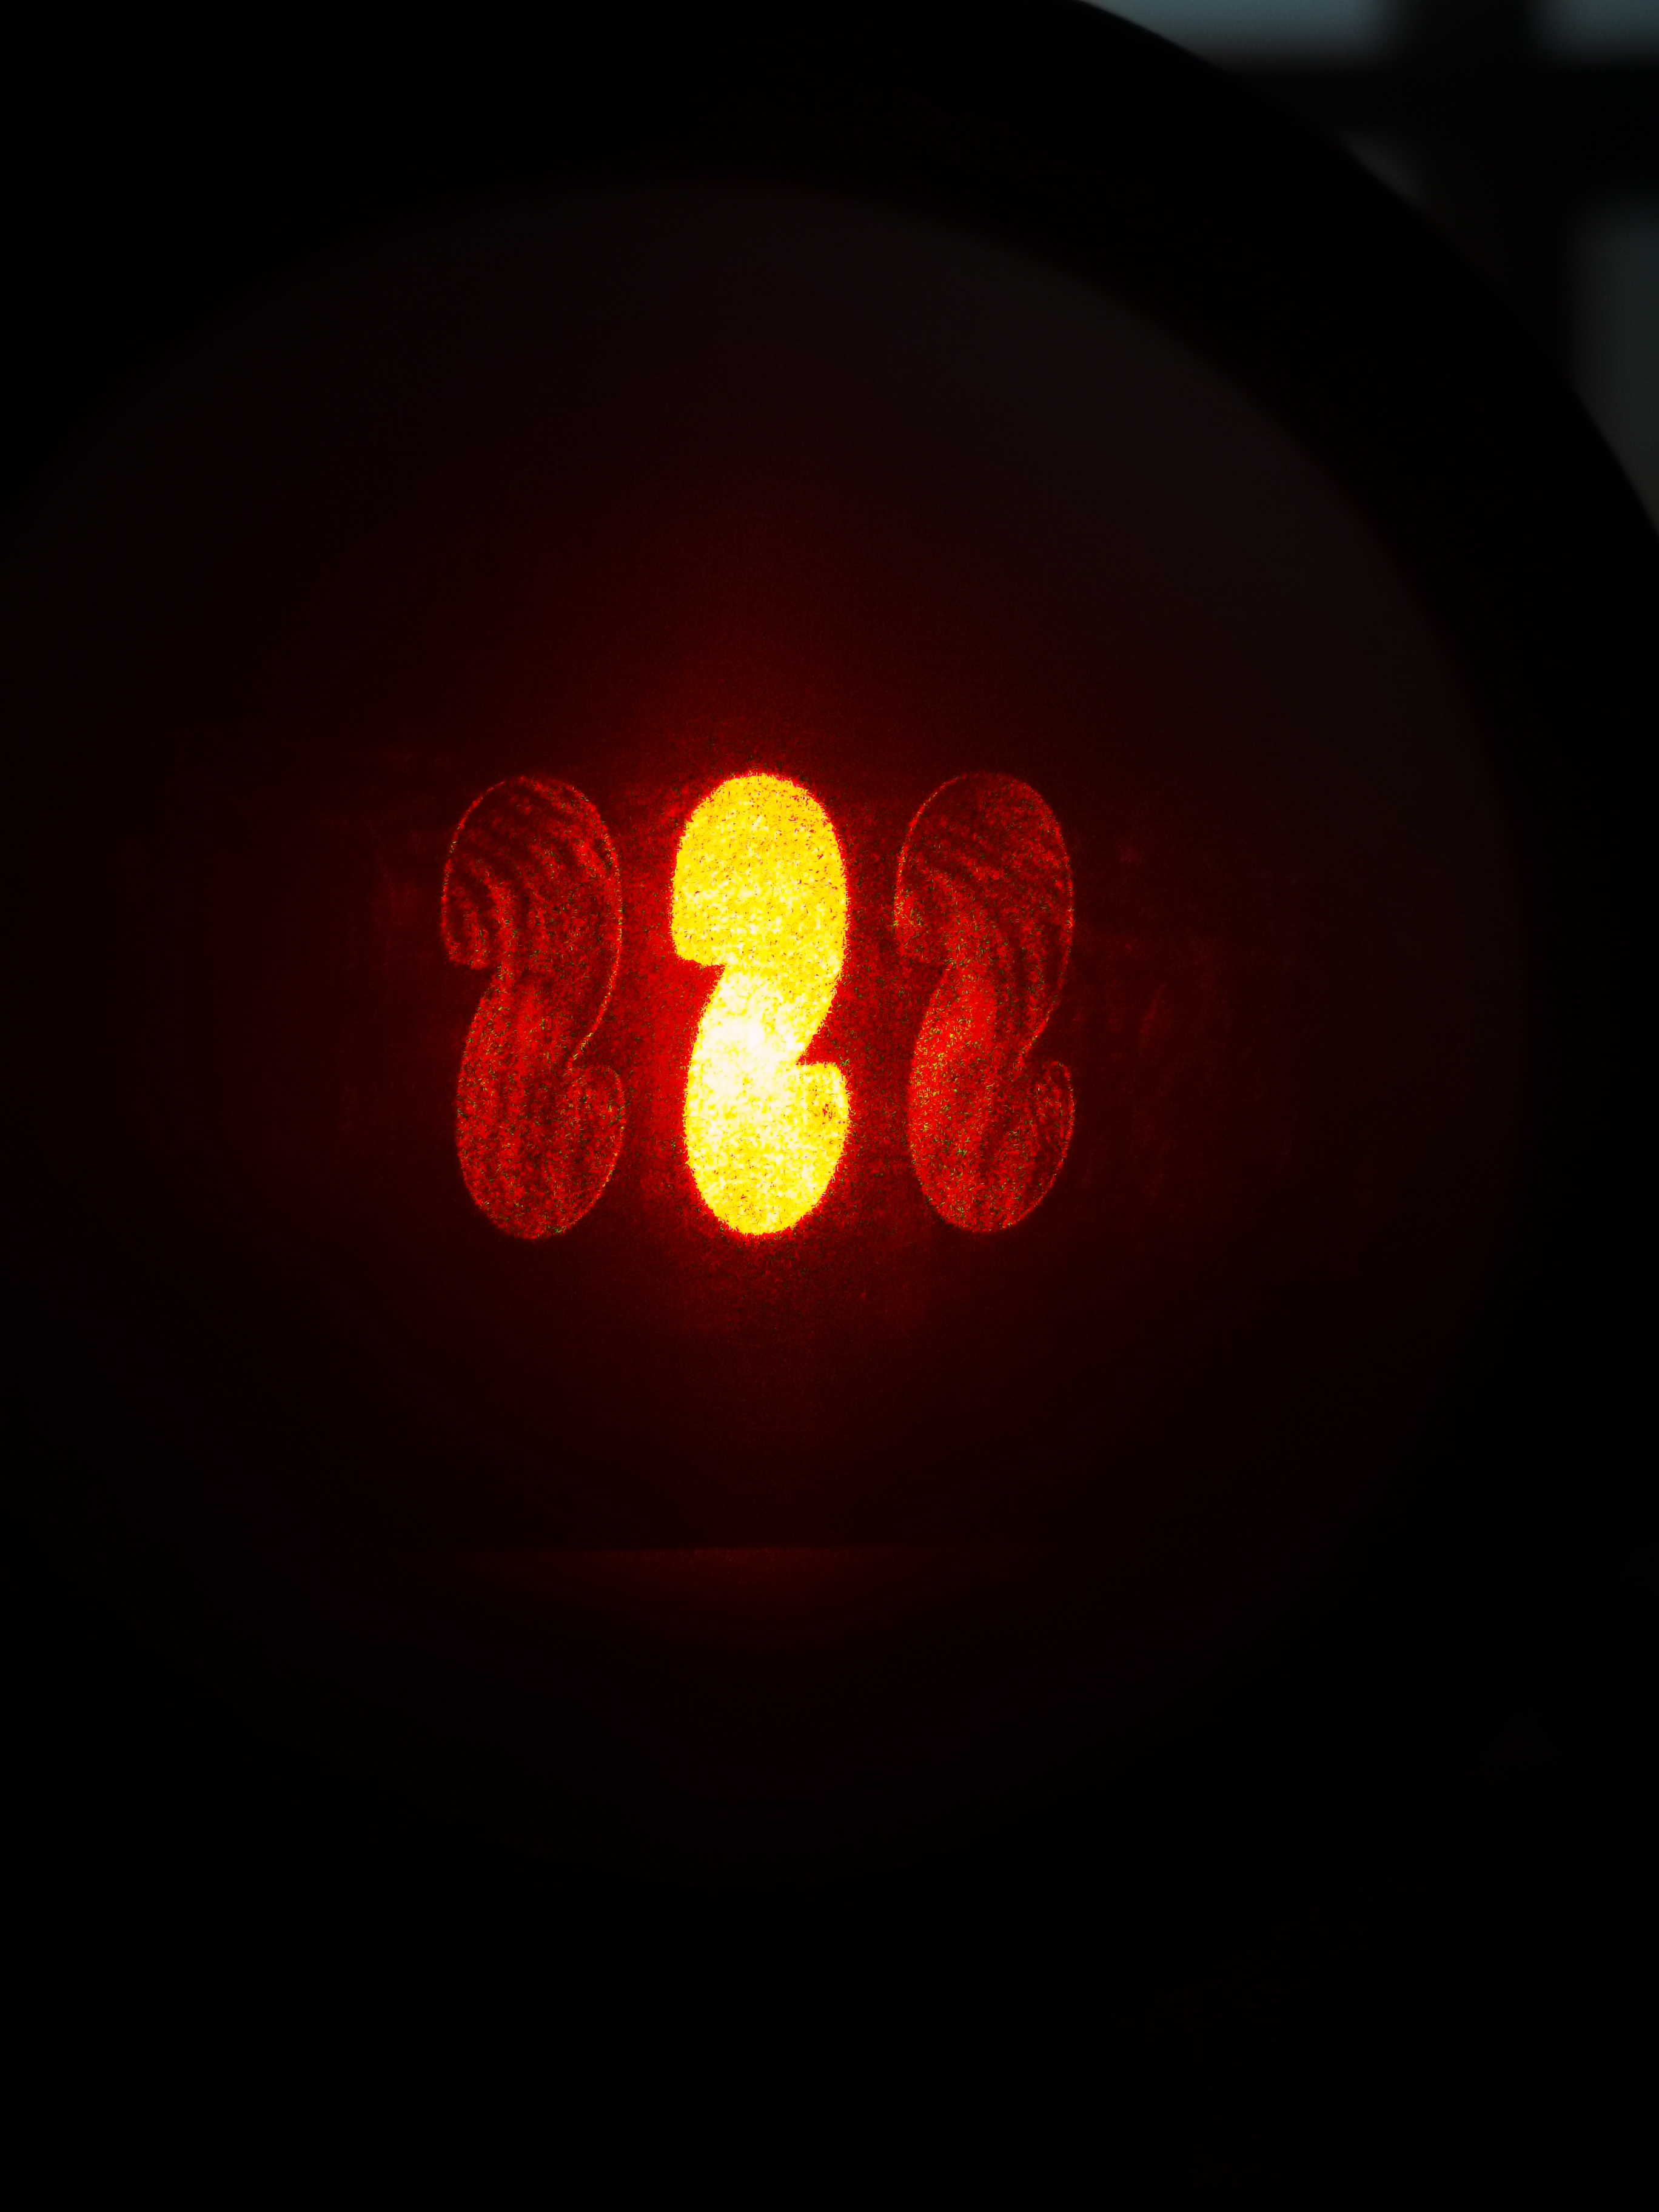
\includegraphics[width=\linewidth]{image/微信图片_20221109232921.jpg}
    \caption{微分后的边缘增强的图像}
    \label{fig:my_label2}
\end{figure}

\begin{figure}
    \centering
    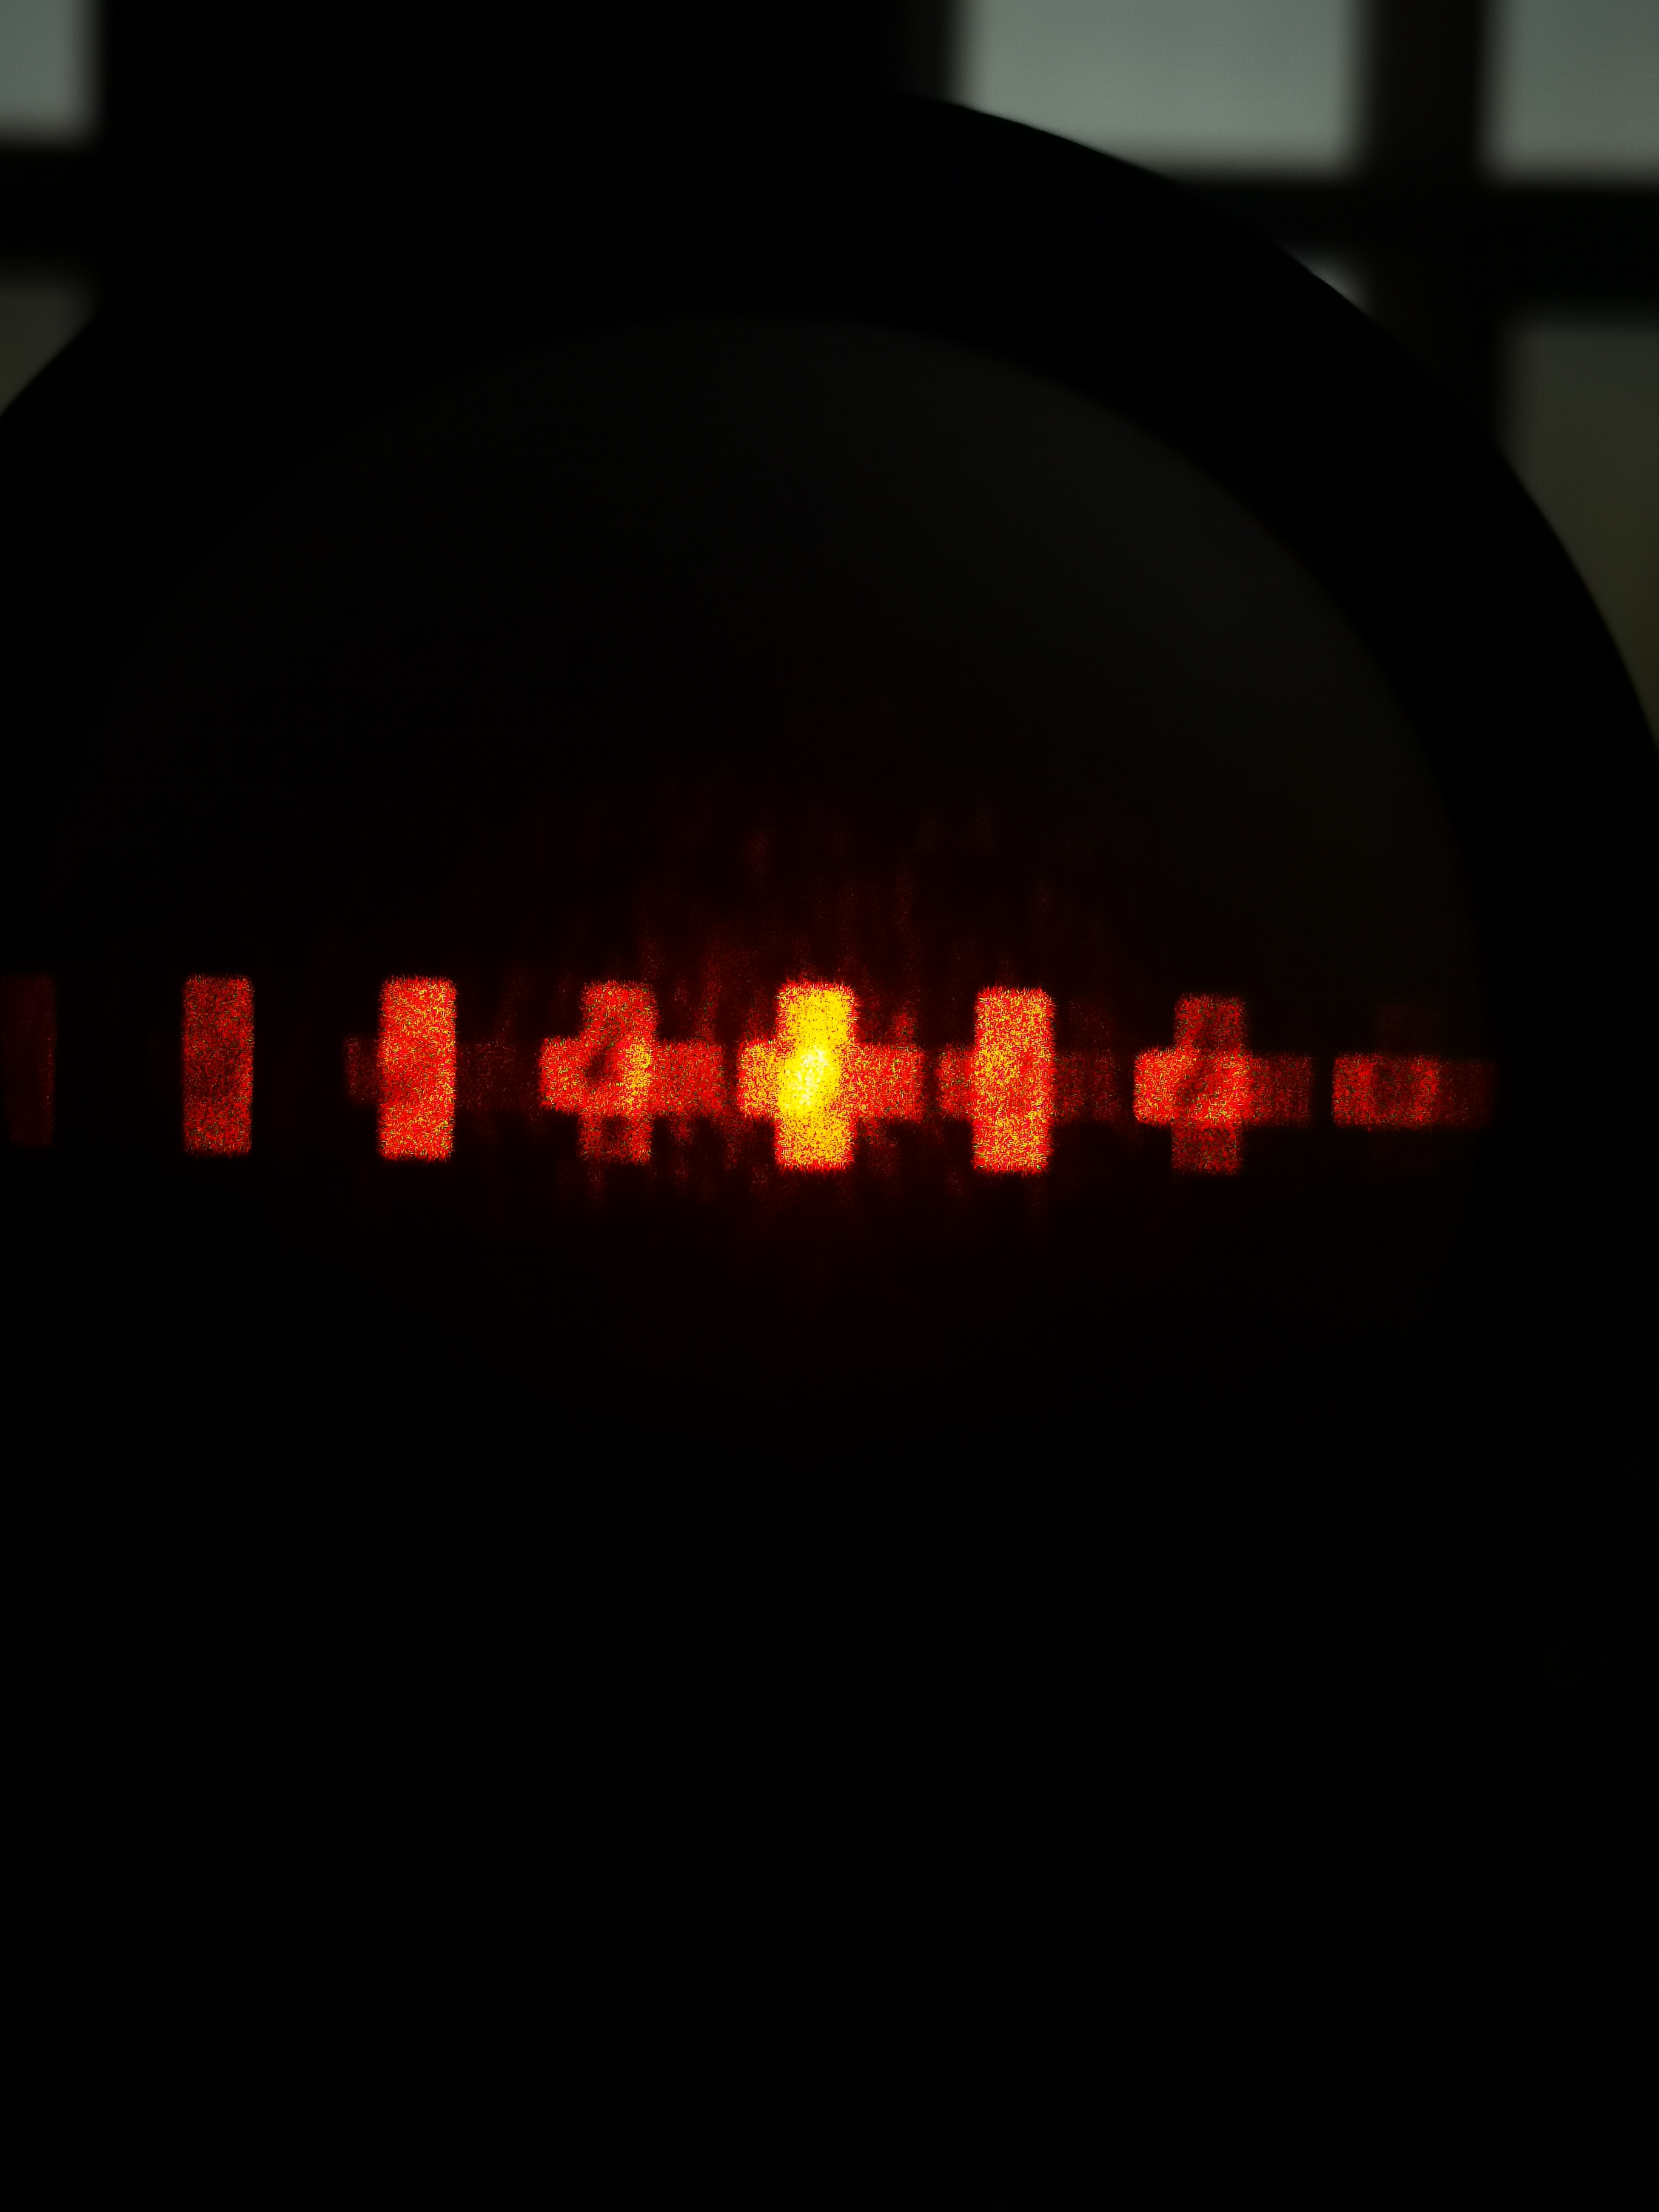
\includegraphics[width=\linewidth]{image/微信图片_202211092329211.jpg}
    \caption{相减后的图像}
    \label{fig:my_label3}
\end{figure}


\section{思~考~题}
\begin{itemize}
    \item 可能是因为两个像的光强不均匀, 造成相减是无法刚好相消。或者是入射光未调成水平。
    \item 由 $\Delta=\frac{1}{4f_0}=\frac{\lambda f}{4b}$,可估计横向位移量级,移动量将增大。
    \item 原理一样,区别在于所用的光栅一个为一维光栅一个为复合光栅。
\end{itemize}

\section{结~~论}
本文利用4f系统来进行光学图像加减和图像微分处理实验,得到了图像的加减和微分图像,同时对光栅的性质和激光器的相关性质有了更为深刻的认识。


%%%%%%%%%%%%%%%%%%%%%%%%%%%%%%%%%%%%%%%%%%%%%%%%%%%%%%%%%%%%%%%%
%  参考文献
%%%%%%%%%%%%%%%%%%%%%%%%%%%%%%%%%%%%%%%%%%%%%%%%%%%%%%%%%%%%%%%%
%  参考文献按GB/T 7714-2015《文后参考文献著录规则》的要求著录. 
%  参考文献在正文中的引用方法:\cite{bib文件条目的第一行}

\renewcommand\refname{\heiti\wuhao\centerline{参考文献}\global\def\refname{参考文献}}
\vskip 12pt

\let\OLDthebibliography\thebibliography
\renewcommand\thebibliography[1]{
  \OLDthebibliography{#1}
  \setlength{\parskip}{0pt}
  \setlength{\itemsep}{0pt plus 0.3ex}
}

{
\renewcommand{\baselinestretch}{0.9}
\liuhao
\bibliographystyle{gbt7714-numerical}
\bibliography{./TempExample}
}


\end{document}
